% !TEX encoding = UTF-8 Unicode

\documentclass[a4paper]{article}

\usepackage{color}
\usepackage{url}
\usepackage[T2A]{fontenc} % enable Cyrillic fonts
\usepackage[utf8]{inputenc} % make weird characters work
\usepackage{graphicx}
\graphicspath{ {slike/} }

\usepackage[english,serbian]{babel}
%\usepackage[english,serbianc]{babel} %ukljuciti babel sa ovim opcijama, umesto gornjim, ukoliko se koristi cirilica

\usepackage[unicode]{hyperref}
\hypersetup{colorlinks,citecolor=green,filecolor=green,linkcolor=blue,urlcolor=blue}

%\newtheorem{primer}{Пример}[section] %ćirilični primer
\newtheorem{primer}{Primer}[section]

\begin{document}

\title{Asembliranje sekvenci\\ \small{Seminarski rad u okviru kursa\\Uvod u bioinformatiku\\ Matematički fakultet}}

\author{Aleksandra Karadžić, Dragutin Ilić\\ karadzic.matf@gmail.com, dragutin\_ilic@yahoo.com}
\date{18.~maj 2017.}
\maketitle

\abstract{
U ovom tekstu je ukratko prikazana osnovna forma seminarskog rada. Obratite pažnju da je pored ove .pdf datoteke, u prilogu i odgovarajuća .tex datoteka, kao i .bib datoteka korišćena za generisanje literature. Na prvoj strani seminarskog rada su naslov, apstrakt i sadržaj, i to sve mora da stane na prvu stranu! Kako bi Vaš seminarski zadovoljio standarde i očekivanja, koristite uputstva i materijale sa predavanja na temu pisanja seminarskih radova. Ovo je samo šablon koji se odnosi na fizički izgled seminarskog rada (šablon koji \emph{morate} da ispoštujete!) kao i par tehničkih pomoćnih uputstava. Molim Vas da kada budete predavali seminarski rad, imenujete datoteke tako da sadrže temu seminarskog rada, kao i imena i prezimena članova grupe (ili samo temu i prezimena, ukoliko je sa imenima predugačko). Predaja seminarskih radova biće isključivo preko web forme, a NE slanjem mejla.

\tableofcontents

\newpage

\section{Uvod}
\label{sec:uvod}

Sekvenciranje genoma, odnosno određivanje rasporeda nukleotida (nt) u genomu, je jedan od fundamentalnih zadataka u bioinformatici. Dužina genoma varira u zavisnosti od organizma (dužina ljudskog genoma je oko 3 milijarde nt, a jedan od najdužih genoma pripada amorfnom jednoćelijskom organizmu \textit{Ameoba dubia} koja je oko 200 puta duži). Najveća prepreka je zapravo činjenica da još uvek nisu razvijene tehnologije koje omogućavaju čitanje nukleotida u genomu od početka do kraja (slično kao čitanje stranica knjige sleva udesno). Trenutno zastupljeno rešenje je sekvenciranje manjih fragmenata DNK koji se nazivaju \textbf{ridovi (\textit{eng. reads})}. Uzima se mali uzorak tkiva ili krvi koji sadrži milione kopija DNK. Biohemijskim procesima se DNK razbija na fragmente, čijim sekvenciranje se dobijaju ridovi. Ne zna se iz kog dela genoma je dobijen određeni rid, pa se koristi tehnika preklapanja ridova da bi se rekontruisao genom. Ovaj ceo proces se naziva i \textbf{asembliranje genoma (\textit{eng. genome assembly})}. \\
\indent Prvo sekvenciranje genoma je odrađeno 1977. godine od strane Frederika Sangera (eng. Frederick Sanger). U Sangerovom metodu dužina ridova je bila između 500 i 1000 ridova. Većina programa zasnovana na ovoj tehnici (\textit{eng. de novo assembly programs}) se bazira na strategiji  "preklapanje-raspored-konsenzus" (\textit{eng. overlap-layout-consensus strategy}), u kojoj se preklapanja između ridova izračunavaju brzim tehinikama upore\-đivanja, raspored kontiga (\textit{eng. contigs}) se generiše pomoću preklapanja u opadajućem rasporedu kvaliteta, a konsenzus sekvenci kontiga se dobija brzim metodama višestrukog poravnavanja. Glavni razlog uspešnosti ovih programa jeste ta da je veličina ridova dovoljna za ustanovljavanje razlika između pravih i lažnih preklapanja. \\
\indent Prilikom sekvenciranja genoma nailazimo na otežavajuće situacije.Prvo, DNK se sastoji od dve niti, pa ne možemo znati iz koje od njih je rid izveden (nemamo inforamciju da li da koristimo dobijen rid ili njegov obrnuti komplement prilikom asembliranja određene niti u genomu). Drugo, tehnologije koje se koriste nisu savršene, pa dobijeni ridovi često sadrže greške (čime se otežava preklapanje ridova). Treće, neki regioni genoma mogu da ostanu nepokriveni ridovima, čime je onemogućena rekonstrukcija celog genoma. Za otklanjanje ovih problema se koriste razne tehnike kao na primer: pristup razbijanja ridova (\textit{eng. read breaking 
approach}) se koristi za problem nepokrivenosti genoma ridovima, asembliranje kontiga (neprkidnih delova genoma), a ne čitavih hromozoma, se vrši zbog navedenih problema,tehnika uklanjanja mehurova (\textit{eng. bubble removal}) kojom se rešavaju ridovi sa greškom (lažni ridovi) itd. \\
\indent Sa ulaskom u drugu genereciju (masovno paralelnih) sekvencijalnih tehnologija, počelo se sa proizvodnjom na milijarde kratkih ridova dužine od 50 do 150 nukleotida. Ogromni skupovi podataka vremenski i prostorno usložnjavaju izra\-čuna\-va\-nje preklapanja dinamičkim algoritmima. Ridovi male dužine otežavaju otkrivanje tačnih od lažnih preklapanja prilikom generisanja rasporeda kontiga. Kako bi se ovo izbeglo, razvijeni su algoritmi za asembliranje zasnovani na detekciji preklapanja kao tačnih pogodataka fiksne dužine. Na osnovu ovakvih preklapanja formira se \textit{de Bruijin}-ov graf, u kome svaki jedinstevni string dužine k (k-mer) koji se pojavljuje u ridu, predstavlja granu koja spaja čvorove označene sa k-1-mer prefiksom i k-1-mer sufiksom. Pomoću ovog grafa i distribucije frekvencije stringova u ridovima razlikujemo stringove koji imaju grešku od onih koji nemaju. Stringovi sa greškama se ili ne koriste ili se prepravljaju i zatim koriste pri asembliranju.  \\
\indent Kako bi koristili sekvenciranje ridova direktno, u ovom radu je predstavljen efikasan metod za izračunjavanje preklapanja za kratke ridove. Metod dozvoljava promašaje u preklapanjima, ali ne dodavanja i brisanja, koji se inače i javljaju ređe od promašaja. U grafu preklapanja, svaki čvor predstavlja rid, dok grana predstavlja preklapanje. U ovom grafu algoritam pronalazi jedinstvenu putanju ridova koja reprezentuje kontigu. Konsenzus sekvence svake kontige je dobijen izračunavanjem poravnanja višestrukih ridova koji nisu razdvojeni nukleotidima koji oni ne sadrže. \\
\indent U nastavku će biti predstavljni detalji algoritma kao i opis programa PCAP.Solexa u kome je algoritam implementiran.
\iffalse
\begin{primer}
Problem zaustavljanja (eng.~{\em halting problem}) je neodlučiv \cite{haltingproblem}.
\end{primer}

\begin{primer}
Za prevođenje programa napisanih u programskom jeziku C može se koristiti GCC kompajler \cite{gcc}.
\end{primer}

\begin{primer}
 Da bi se ispitivala ispravost softvera, najpre je potrebno precizno definisati njegovo ponašanje \cite{laski2009software}. 
\end{primer}
Reference koje se koriste u ovom tekstu zadate su u datoteci {\em seminarski.bib}. Prevođenje u pdf format u Linux okruženju može se uraditi na sledeći način:

\begin{verbatim}
pdflatex TemaImePrezime.tex 
bibtex TemaImePrezime.aux 
pdflatex TemaImePrezime.tex 
pdflatex TemaImePrezime.tex 
\end{verbatim}
Prvo latexovanje je neophodno da bi se generisao {\em .aux} fajl. {\em bibtex} proizvodi odgovarajući {\em .bbl} fajl koji se koristi za generisanje literature. 
Potrebna su dva prolaza (dva puta pdflatex) da bi se reference ubacile u tekst (tj da ne bi ostali znakovi pitanja umesto referenci). Dodavanjem novih referenci potrebno je ponoviti ceo postupak.  


Broj naslova i podnaslova je proizvoljan. Neophodni su samo Uvod i Zaključak. Na poglavlja unutar teksta referisati se po potrebi. 
\begin{primer}
U odeljku \ref{sec:naslov1} precizirani su osnovni pojmovi, dok su zaključci dati u odeljku \ref{sec:zakljucak}.
\end{primer}

\fi



\section{Opis algoritma}
\label{opis_algoritma}
Na početku ćemo opisati metod koji se koristi za izračunavanje preklapanja izmedju ridova. Za realizaciju ovog metoda je korišćena struktura podataka koju ćemo zvati \textbf{``niz super-reč''} (\textit{eng. superword array}), koja je ime dobila na sličan način kao i druga struktura podataka zvana ``sufiksni niz'' (\textit{eng. sufix array}). Reč dužine \textit{w} je string od \textit{w} karaktera, a super-reč sa \textit{v} reči je string sa \textit{v*w} karaktera dobijena konkatenacijom tih reču po redu u kome se javljaju. Reči u super-reči ćemo indeksirati pozicijama od 1 do \textit{v}. Pozicije u rečima (indeksiranje kreće od jedinice) se dele u dve grupe: čekirane i nečekirane poicije. Za dve reči dužine \textit{w} kažemo da se podudaraju ukoliko imaju identične nukleotide na svakoj čekiranoj poziciji tih reči. Na primer ako imamo dve reči dužine 15, \textbf{ACCATACCATAGCAC} i \textbf{ACTATTCCATAACAC}, i ako pretpostavimo da su nečekirane pozicije 3,6 i 12 tada za ove dve reči možemo reći da se podudaraju. Dužina reči \textit{w} se često namešta da bude 12 ili veća, kako bi broj čekiranih pozicija u reči bio 12, čime se osigurava da lookup tabela za sve stringove ove dužine (ako je reč duža od 12 brišemo sve nukleotide iz nečekiranih pozicija) može stati u glavnu memoriju. Broj reči \textit{v} se bira tako da super-reč dužine \textit{v*w} bude manja od dužine svakog rida (dužinu rida ćemo označavati sa  \textit{r}). Dužina super-reči se još naziva i minimalna dužina preklapanja. Adekvatan primer za ridove dužine 150 bi bio da postavimo da \textit{w} na 15 i \textit{v} na 6 čime dobjamo super-reči dužine 90. Rid dužine \textit{r} ima \textit{r - w*v }+ 1 super-reči na pozicijama 1,2, \ldots ,\textit{r - w*v }+ 1. U našem primeru bi rid dužine 150 imao 61 super-reč na pozicijama 1,2, \ldots ,61. Za dve super-reči kažemo da su identične ako im se sve reči podudaraju, odnosno svi nukleotidi na čekiranim pozcijama su im identični. Za jednu super-reč kažemo da je manja (veća) od druge ako string nukleotida na svakoj čekiranoj poziciji prve super-reči, u lekiskografskom poredku, dolazi pre (posle) stringa nukleotida na čekiranim pozicijama druge super-reči. Svaki rid dobija jedinstveni nenegativni ceo broj koji se zove indeks rida. Pomoću njega i početne pozicije super-reči u ridu se izračunava indeks svake super-reči u svakom ridu. U algoritmu se koristi i funkcija koja pomoću datog indeksa super-reči računa efikasno računa poziciju te super-reči u indeksu i indeks rida.Sada imamo sve podatke kako bi definisali ``niz super-reč'' strukturu podataka. \textbf{``niz super-reč''} za skup ridova je niz svih indeksa super-reči gde su super-reči sortirane od manje ka većoj.

\begin{figure}[h!]
\begin{center}
\end{center}
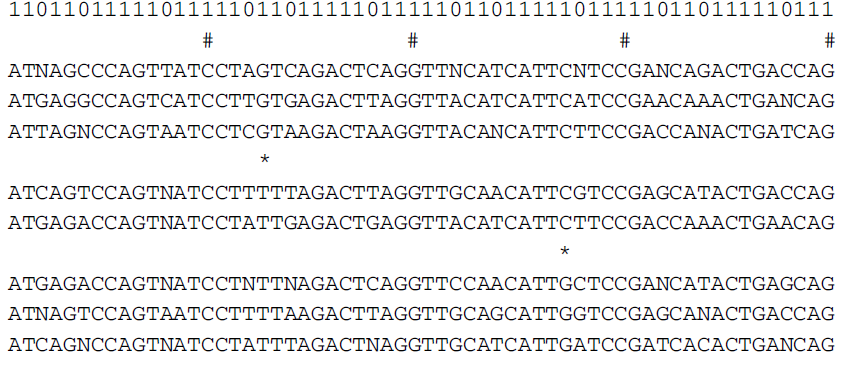
\includegraphics[width=\textwidth]{superreci}
\label{fig:superreci}
\caption{Prikaz super-reči}
\end{figure}

\indent Na slici \ref{fig:superreci} prikazano je osam super-reči u sortiranom poredku. Svaka super-reč se sastoji od četiri reči (v=4) dužine w = 15, gde je svaka čekirana pozicija označena bitom 1 , a nečekirana 0. Poslednja pozicija svake reči je označena taraba znakom. Super-reči su grupisane tako da se u svakom bloku nalaze identične super-reči (prve tri, sledeće dve i poslednje tri). Vidimo da nukleotidi na nečekiranim pozicijama mogu biti različiti u istom bloku ili biti nedefinisani (označeni sa \textbf{N}). Pvi blok dolazi pre drugog zato što na poziciji označenoj sa zvezdicom se u prvom bloku nalazi \textbf{G} nukleotid a u drugom \textbf{T} (\textbf{G} leksikografski dolazi pre \textbf{T}). Slično zvezdica izmedju drugog i trećeg bloka označava zašto drugi dolazi pre trećeg.

\iffalse
Slike i tabele treba da budu u svom okruženju, sa odgovarajućim naslovima, obeležene labelom da koje omogućava referenciranje. 

\begin{primer} Ovako se ubacuje slika. Obratiti pažnju da je dodato i 
\begin{verbatim}
\usepackage{graphicx}
\end{verbatim}

%\begin{figure}[h!]
%\begin{center}
%\end{center}
%\caption{Pande}
%\label{fig:pande}
%\end{figure}

%Na svaku sliku neophodno je referisati se negde u tekstu. Na primer, na slici \ref{fig:pande} prikazane su pande. 
\end{primer}

\begin{primer} I tabele treba da budu u svom okruženju, i na njih je neophodno referisati se u tekstu. Na primer, u tabeli \ref{tab:tabela1} su prikazana različita poravnanja u tabelama.

\begin{table}[h!]
\begin{center}
\caption{Razlčita poravnanja u okviru iste tabele ne treba koristiti jer su nepregledna.}
\begin{tabular}{|c|l|r|} \hline
centralno poravnanje& levo poravnanje& desno poravnanje\\ \hline
a &b&c\\ \hline
d &e&f\\ \hline
\end{tabular}
\label{tab:tabela1}
\end{center}
\end{table}

\end{primer}

\fi



\section{Prvi naslov}
\label{sec:naslov1}


Ovde pišem tekst. 
Ovde pišem tekst. 
Ovde pišem tekst. 
Ovde pišem tekst. 
Ovde pišem tekst. 
Ovde pišem tekst. 
Ovde pišem tekst. 
Ovde pišem tekst. 


\subsection{Prvi podnaslov}
\label{subsec:podnaslov1}

Ovde pišem tekst. 
Ovde pišem tekst. 
Ovde pišem tekst. 
Ovde pišem tekst. 
Ovde pišem tekst. 
Ovde pišem tekst. 
Ovde pišem tekst. 

\subsection{Drugi podnaslov}
\label{subsec:podnaslov2}

Ovde pišem tekst. 
Ovde pišem tekst. 
Ovde pišem tekst. 
Ovde pišem tekst. 
Ovde pišem tekst. 
Ovde pišem tekst. 

\section{Drugi naslov}
\label{sec:naslov2}

Ovde pišem tekst. 
Ovde pišem tekst. 
Ovde pišem tekst. 
Ovde pišem tekst. 

\subsection{... podnaslov}
\label{subsec:podnaslovN}

Ovde pišem tekst. 
Ovde pišem tekst. 
Ovde pišem tekst. 
Ovde pišem tekst. 
Ovde pišem tekst. 
Ovde pišem tekst. 

\section{n-ti naslov}
\label{sec:naslovN}

Ovde pišem tekst. 
Ovde pišem tekst. 
Ovde pišem tekst. 
Ovde pišem tekst. 
Ovde pišem tekst. 

\subsection{... podnaslov}
\label{subsec:podnaslovK}

Ovde pišem tekst. 
Ovde pišem tekst. 
Ovde pišem tekst. 
Ovde pišem tekst. 
Ovde pišem tekst. 

\subsection{... podnaslov}
\label{subsec:podnaslovM}

Ovde pišem tekst. 
Ovde pišem tekst. 
Ovde pišem tekst. 
Ovde pišem tekst. 
Ovde pišem tekst. 

\section{Poslednji naslov}
\label{sec:naslovM}

Ovde pišem tekst. 
Ovde pišem tekst. 
Ovde pišem tekst. 
Ovde pišem tekst. 
Ovde pišem tekst. 
Ovde pišem tekst. 
Ovde pišem tekst. 
Ovde pišem tekst. 
Ovde pišem tekst. 

\section{Zaključak}
\label{sec:zakljucak}

Ovde pišem zaključak. 
Ovde pišem zaključak. 
Ovde pišem zaključak. 
Ovde pišem zaključak. 
Ovde pišem zaključak. 
Ovde pišem zaključak. 
Ovde pišem zaključak. 
Ovde pišem zaključak. 
Ovde pišem zaključak. 
Ovde pišem zaključak. 
Ovde pišem zaključak. 
Ovde pišem zaključak. 


\addcontentsline{toc}{section}{Literatura}
\appendix
\bibliography{seminarski} 
\bibliographystyle{plain}

\appendix
\section{Dodatak}
Ovde pišem dodatne stvari, ukoliko za time ima potrebe.
Ovde pišem dodatne stvari, ukoliko za time ima potrebe.
Ovde pišem dodatne stvari, ukoliko za time ima potrebe.
Ovde pišem dodatne stvari, ukoliko za time ima potrebe.
Ovde pišem dodatne stvari, ukoliko za time ima potrebe.


\end{document}
